\chapter{Desarrollo}

	A continuaci\'on se describe de forma detallada, el diseño y desarrollo del paquete \textbf{apnnClassifier} para la clasificaci\'on de tub\'erculos de papa criolla(\textit{Solanum phureja}) para diferentes densidades de siembra empleando redes neuronales probabil\'isticas, siguiendo la metodolog\'ia descrita en el cap\'itulo 3.
	
\section{Creación del esqueleto del paquete.}
	
	Para esta fase se utilizó el ambiente de desarrollo RStudio, el cual es un entorno de desarrollo integrado de fuente abierta para R que agrega muchas caracter\'isticas y herramientas de productividad, además de facilitar el uso de R integrando la ayuda y la documentación.\\
En esta primera etapa se creó la estructura del paquete, la cual esta conformada por la identificación por nombre y descripción del paquete(Figura 4.1), además, se cargan los paquetes del CRAN de R y sus extensiones, de los cuales dependen los metodos y funciones que permitiran el desarrollo del paquete apnnClassifier; los mismos fueron almacenados en el repositorio local que se crea para este paquete durante el proceso de desarrollo; los principales fueron:\\

\begin{itemize}
\item pnn(Chasset, P. \textit{et. al}, 2013; https://cran.r-project.org/web/packages/pnn/index.html)
\item pROC(Robin, X. \textit{et. al}, 2019; https://cran.r-project.org/web/packages/pROC/index.html)
\item dplyr(Wickham, H. \textit{et. al}, 2019; https://cran.r-project.org/web/packages/dplyr/index.html)
\item roxygen2(Ooms, J. \textit{et. al}, 2018; https://cran.r-project.org/web/packages/roxygen2/index.html)
\end{itemize}

\begin{figure}[h]
	\caption{Descripción del paquete}
	\centering
	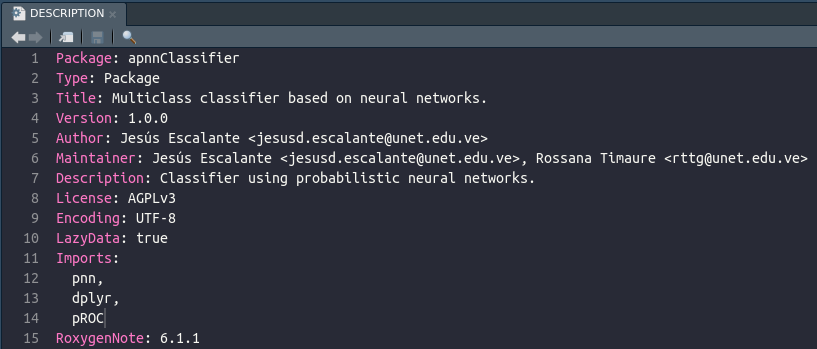
\includegraphics[scale=0.5]{package-description.png}
	\label{fig:arch}
\end{figure}

\section{Diseño de las soluciones algorítmicas para el entrenamiento de una red neuronal probabilística que permita la clasificación de tubérculos de papa.}

	El objetivo funcional del paquete desarrollado es permitir al usuario realizar el entrenamiento de una red neuronal probabilística para la clasificación de datos estandarizados o no estandarizados, así como graficar y evaluar los resultados de la clasificación.\\

	Para este fin se desarrollaron 2 funciones necesarias para llegar a los resultados esperados y una opcional para estandarizar los datos de entrada. \\

	Como entrada para iniciar el proceso de entrenamiento y clasificación, es necesario tener un set de datos de entrenamiento en una estructura data frame, teniendo bien conocida cual es la columna clase del set; así como tener un set de datos de entrenamiento en forma de matriz con la misma cantidad de columnas como variables clasificadoras tenga el set de entrenamiento.\\

	Las funciones antes mencionadas junto a sus entradas, salidas y diagramas de flujos serán descritas a continuación.\\


\section{Diseño del algoritmo de la función de entrenamiento y clasificación de la red (trainNeuralNet).}

	Para el caso de la creación y entrenamiento de la red neuronal probabilística para permitir la clasificación de los datos, se diseñó el ingreso de los datos en dos sets, uno de entrenamiento con la columna de clase incluida y un set de testing con la misma cantidad de datos de entrenamiento que el primer set, además de, el índice de la columna indicadora de clase en el set de entrenamiento y el valor 
óptimo de la función de activación en caso de conocerse (\ref{tabla:entradasTrainNeuralNet}. Pag.\pageref{tabla:entradasTrainNeuralNet}). La función diseñada hace uso del paquete PNN (Chasset, P) de R para crear y entrenar una red neuronal probabilística, el algoritmo de la función se encarga de crear, entrenar, optimizar y clasificar los datos del set de pruebas recibido, obteniendo al final una red neuronal entrenada capaz de clasificar y lista para ser evaluada junto a su clasificación (\ref{fig:trainNeuralNet}. Pag.\pageref{fig:trainNeuralNet}).\\

\begin{table}[htb]
\begin{center}
\begin{tabular}{|p{3cm}|p{5cm}|p{8cm}|}
\hline
\multicolumn{3}{|c|}{\textbf{Entradas}} \\
\hline
\textbf{Nombre} & \textbf{Descripción} & \textbf{Reglas} \\
\hline \hline
train\_set & Set de entrenamiento & Parámetro de tipo dataframe. Requerido. \\ \hline
test\_set & Set de pruebas & Parámetro de tipo matriz. Requerido. \\ \hline
category\_column & Índice de la columna que identifica la categoría o clase en el set de entrenamiento & Parámetro de tipo entero. No requerido. Valor por defecto: 1. \\ \hline
sigma & Valor óptimo de la función de activación & Parámetro de tipo flotante. No requerido. Es calculado en caso de ausencia del parámetro. \\ \hline
\end{tabular}
\caption{Entradas de la función de entrenamiento - \textbf{trainNeuralNet}.}
\label{tabla:entradasTrainNeuralNet}
\end{center}
\end{table}

\begin{figure}[h]
	\caption{Diagrama de flujo para función de entrenamiento y clasificación de la red neuronal probabilística}
	\centering
	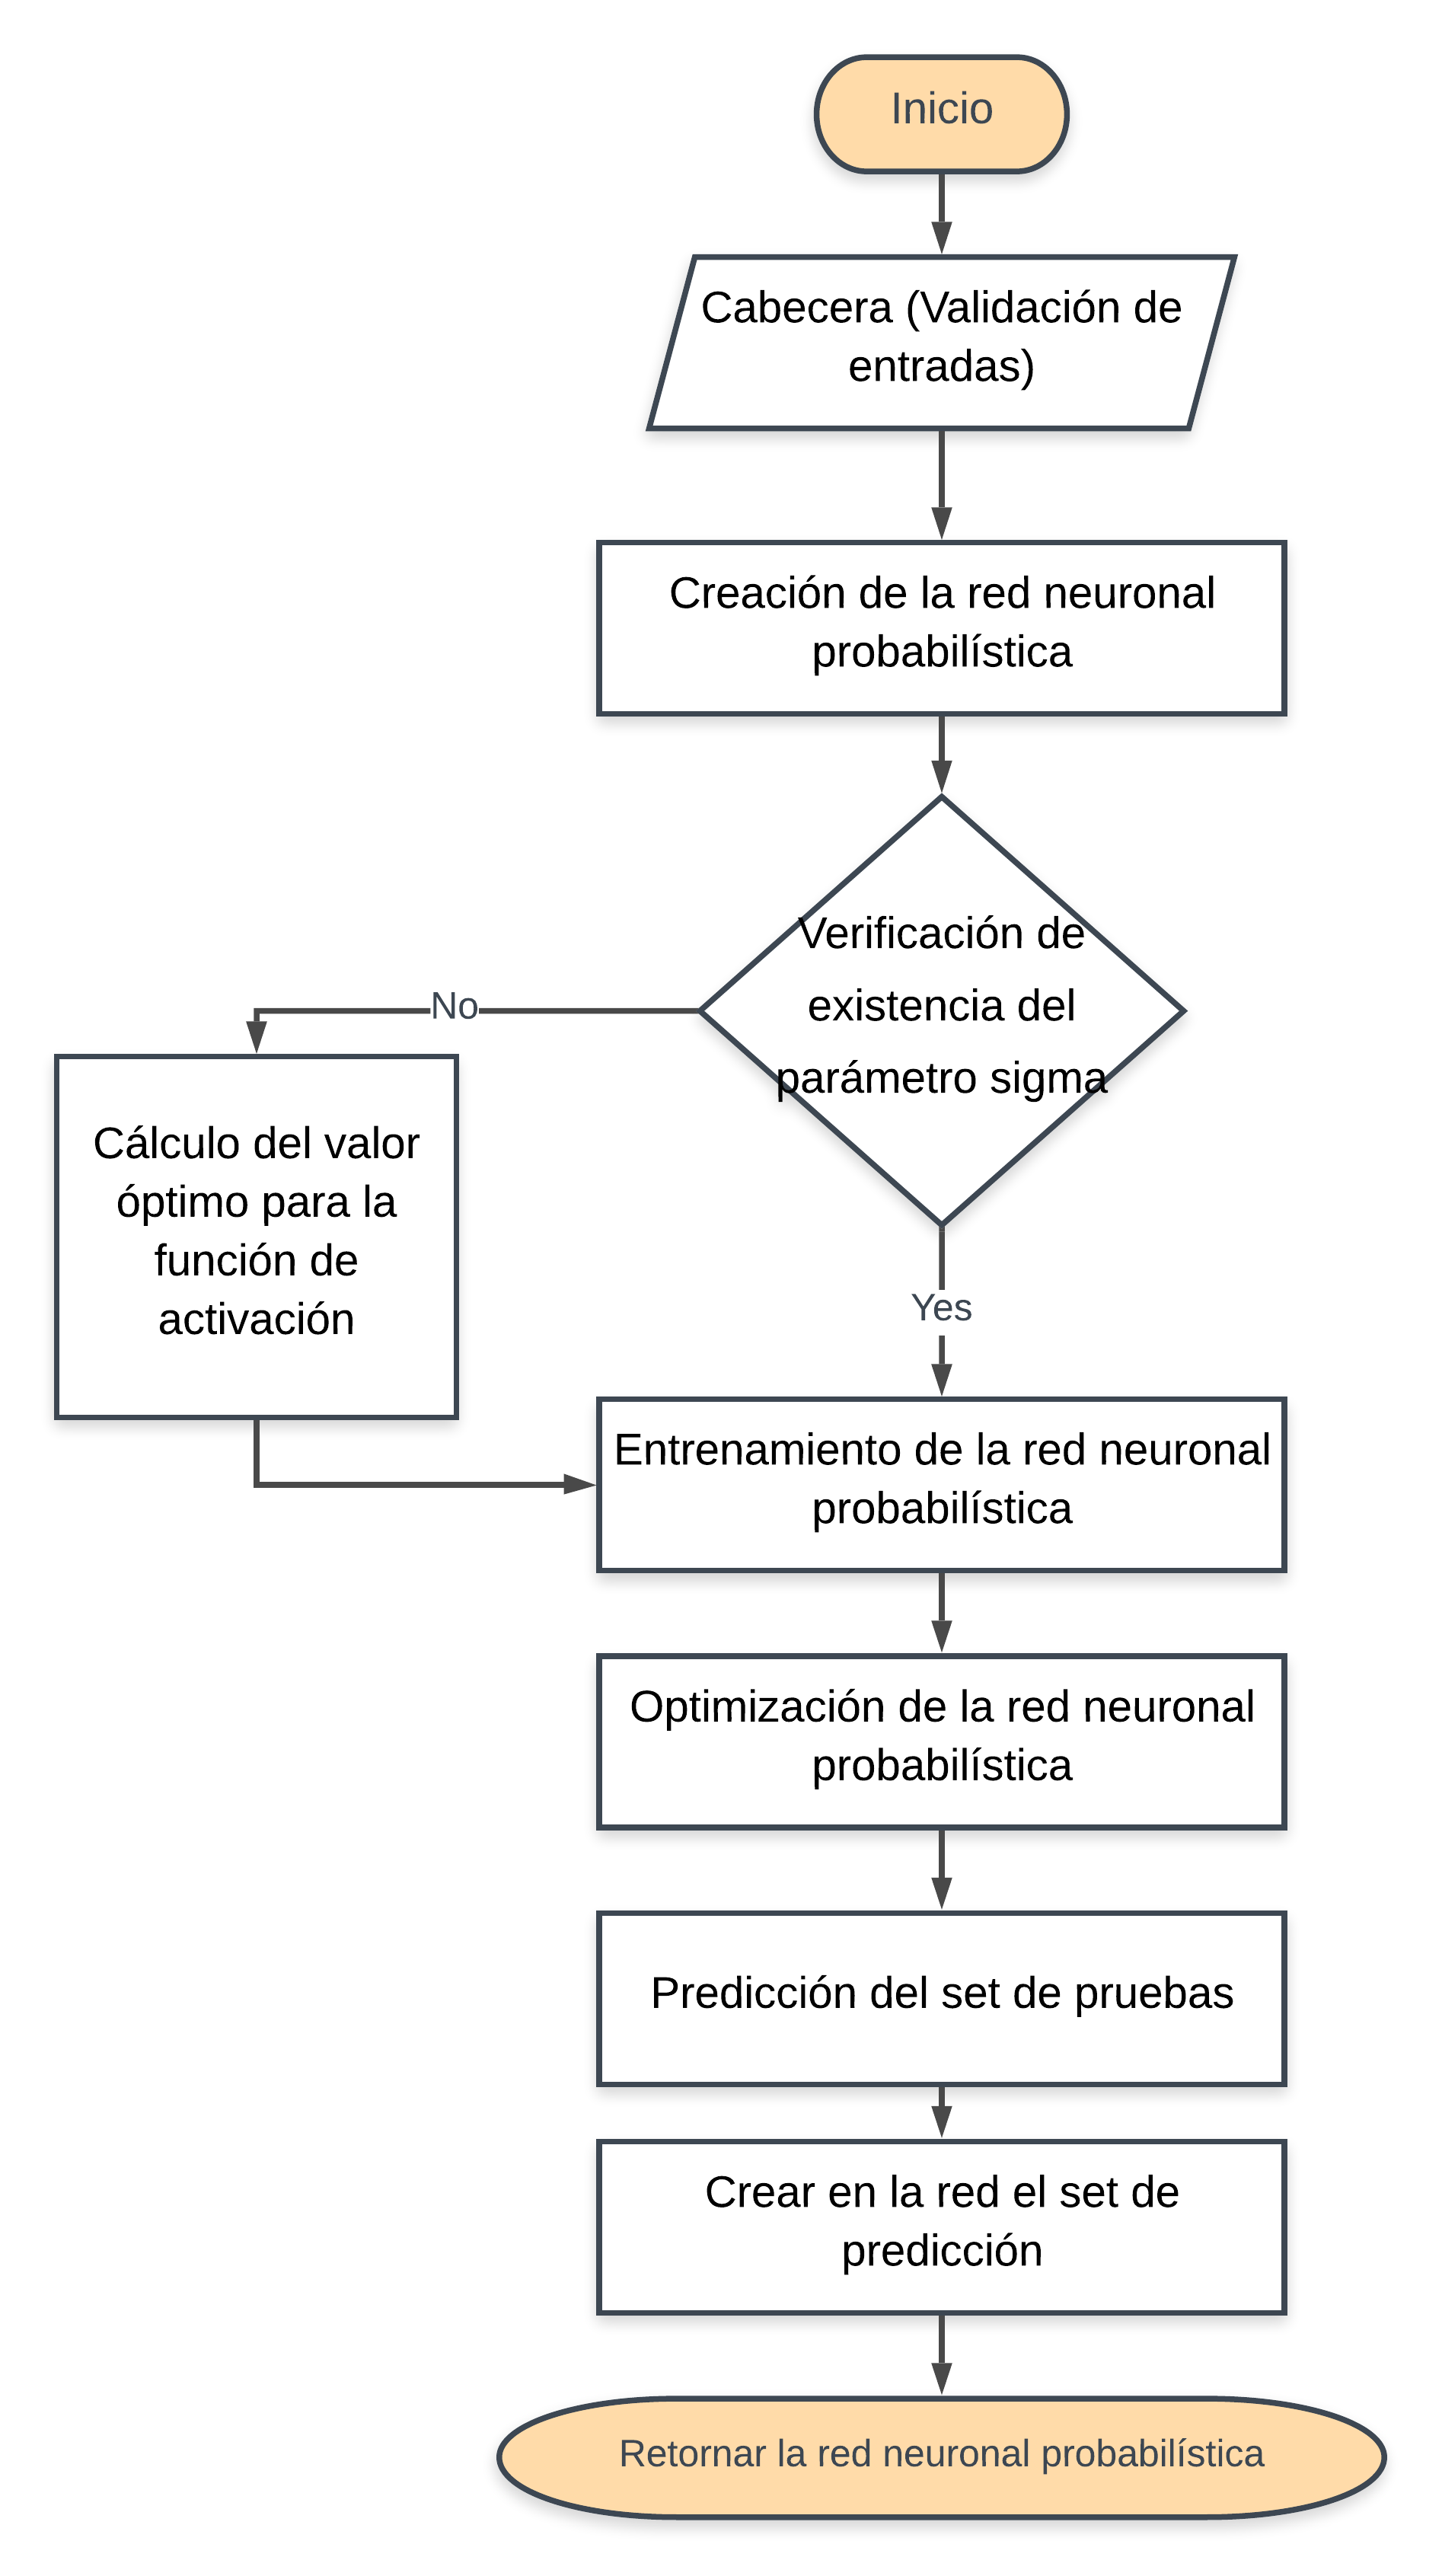
\includegraphics[scale=0.1]{trainNeuralNet.png}
	\label{fig:trainNeuralNet}
\end{figure}

\section{Diseño del algoritmo de la función de evaluación de la red neuronal probabilística y su clasificación (evaluate).}

	Para el caso de la evaluación de la red neuronal probabilística y su clasificación, se unificó el ingreso de los datos en la lista de R que se traduce a la red neuronal probabilística que es salida de la función \textit{trainNeuralNet}, descrita anteriormente (\ref{tabla:entradasEvaluate}. Pag.\pageref{tabla:entradasEvaluate}). La función diseñada realiza la creación del gráfico de nubes de puntos, para demostrar la correlación entre las variables de entrenamiento y hace uso del paquete pROC (Robin, X) de R para crear el gráfico de curvas características operativas (Curvas ROC) para identificar si la clasificación fue buena, el algoritmo también permite observar datos de análisis de la red como su sensibilidad, efectividad y área bajo la curva, para determinar un mal o un buen análisis (\ref{fig:evaluate}. Pag.\pageref{fig:evaluate}).\\

\begin{table}[htb]
\begin{center}
\begin{tabular}{|p{3cm}|p{5cm}|p{8cm}|}
\hline
\multicolumn{3}{|c|}{\textbf{Entradas}} \\
\hline
\textbf{Nombre} & \textbf{Descripción} & \textbf{Reglas} \\
\hline \hline
pnn & Red neuronal probabilística & Parámetro de tipo lista, que es salida de la función descrita en la sección 4.3. Requerido. \\ \hline
\end{tabular}
\caption{Entradas de la función de evaluación - \textbf{evaluate}.}
\label{tabla:entradasEvaluate}
\end{center}
\end{table}

\begin{figure}[h]
	\caption{Diagrama de flujo para función de evaluación de la red neuronal probabilística}
	\centering
	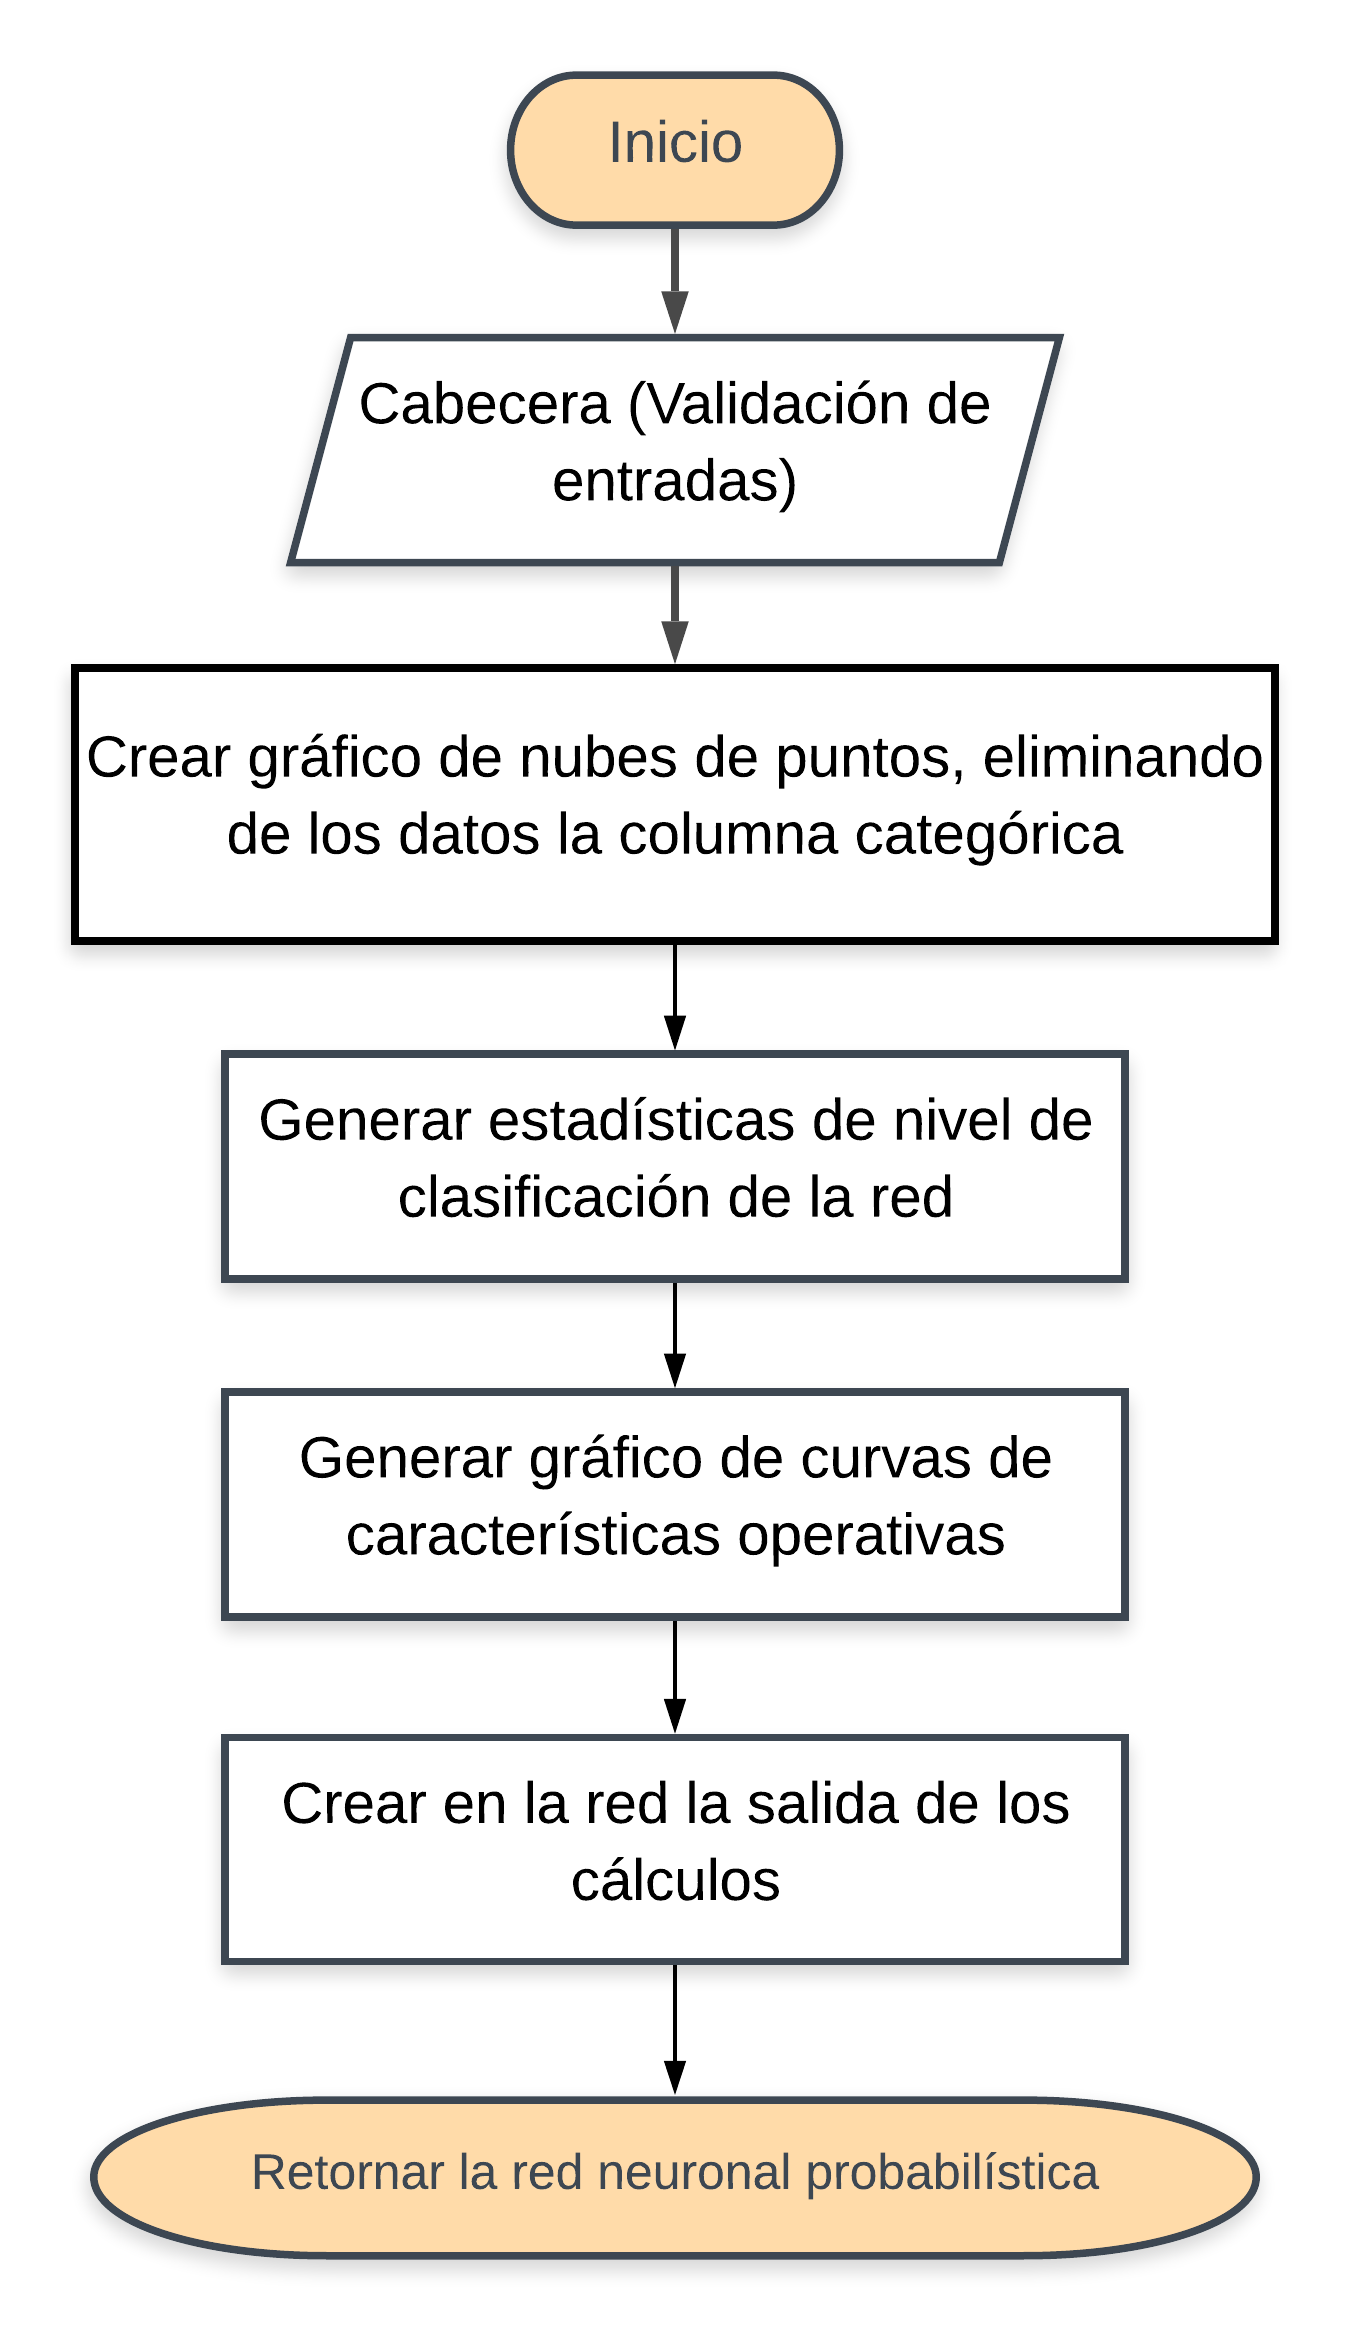
\includegraphics[scale=0.5]{evaluate.png}
	\label{fig:evaluate}
\end{figure}

	La predicción del set de pruebas se puede observar en el atributo “output” de la red neuronal devuelta por la función y es un data frame con dos columnas, una que tiene la predicción y otra con la probabilidad con la que se obtuvo dicha predicción, como se puede observar en la figura \ref{fig:outputTesting}. Pag \pageref{fig:outputTesting}.\\
	
\begin{figure}[h]
	\caption{Ejemplo de predicción de set de pruebas.}
	\centering
	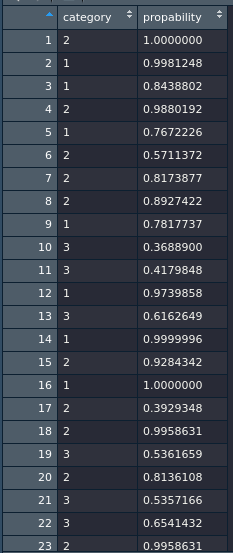
\includegraphics[scale=0.5]{outputTesting.png}
	\label{fig:outputTesting}
\end{figure}

\section{Diseño del algoritmo de la función de estandarización de datos (standardize).}

	Para el caso de la estandarización opcional de los datos, se diseñó el ingreso de los datos en un set en formato lista o data frame, para este paso se debe tener en cuenta que no tiene sentido alguno estandarizar la columna clase. El tipo de estandarización a usar, que puede ser puntual por media y varianza o escalar por minimos y maximos (Tabla: \ref{tabla:entradasStandardize}. Pag.\pageref{tabla:entradasStandardize}). La función diseñada dependiendo del tipo de estandarización indicado en la entrada, aplica la función de estandarización columna por columna del set.(\ref{fig:standardize}. Pag.\pageref{fig:standardize}).\\
	
\begin{table}[htb]
\begin{center}
\begin{tabular}{|p{3cm}|p{5cm}|p{8cm}|}
\hline
\multicolumn{3}{|c|}{\textbf{Entradas}} \\
\hline
\textbf{Nombre} & \textbf{Descripción} & \textbf{Reglas} \\
\hline \hline
set & Set de datos & Parámetro de tipo lista o data frame. Requerido. \\ \hline
type & Tipo de estandarización & Parámetro de tipo cadena de caracteres. No requerido. Valores posibles: "punctual" - "scale". Valor por defecto: "punctual".\\ \hline
\end{tabular}
\caption{Entradas de la función de estandarización - \textbf{evaluate}.}
\label{tabla:entradasStandardize}
\end{center}
\end{table}

\begin{figure}[h]
	\caption{Diagrama de flujo para función de  estandarización de datos}
	\centering
	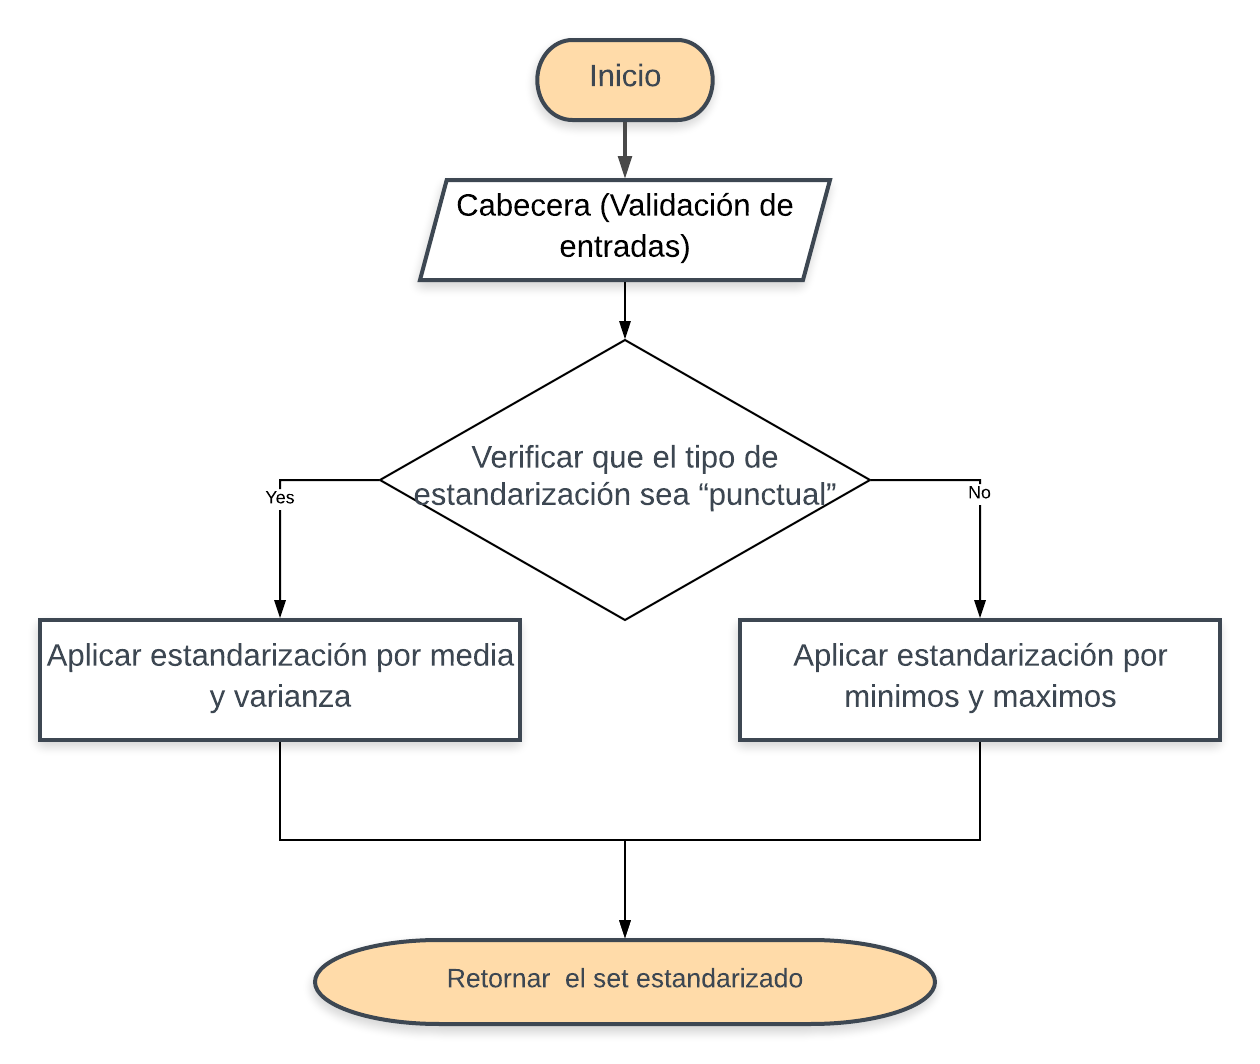
\includegraphics[scale=0.5]{standardize.png}
	\label{fig:standardize}
\end{figure}

\section{Codificación de los algoritmos}

	La codificación de los algoritmos se realizo en el IDE(Entorno de desarrollo integrado) RStudio, siguiendo las especificaciones algoritmicas detalladas con anterioridad.\\

	A continuación se describen las principales funciones creadas para el paquete apnnClassifier.\\
	
\begin{itemize}
\item \textbf{Función de entrenamiento y clasificación de la red \textit{(trainNeuralNet)}}, crea y entrena una red neuronal probabilística y depende del paquete de R Pnn, la codificación de dicha función se muestra en la figura \ref{fig:codeTrainNeuralNet}. Pag \pageref{fig:codeTrainNeuralNet}.

\begin{figure}[h]
	\caption{Codificación de la función de entrenamiento y clasificación de la red neuronal probabilística.}
	\centering
	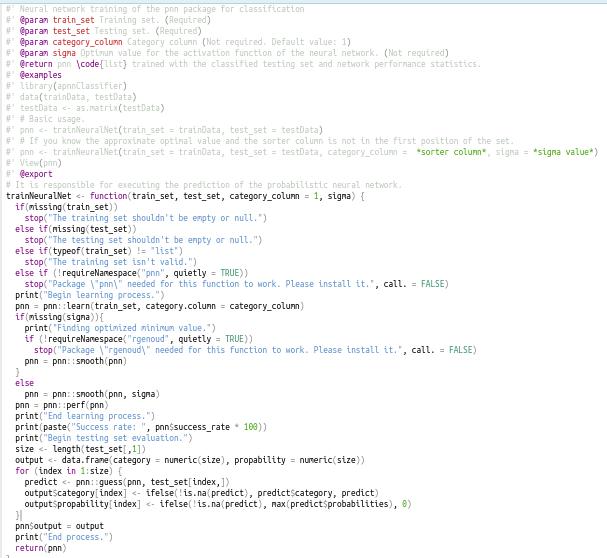
\includegraphics[scale=0.5]{codeTrainNeuralNet.png}
	\label{fig:codeTrainNeuralNet}
\end{figure}

\item \textbf{Función de evaluación de la red \textit{(evaluate)}}, evalua la especificidad, efectividad y sensibilidad de la clasificación realizada por la red neuronal probabilística y depende del paquete de R pROC y dPlyr, la codificación de dicha función se muestra en la figura \ref{fig:codeEvaluate}. Pag \pageref{fig:codeEvaluate}.

\begin{figure}[h]
	\caption{Codificación de la función de evaluación de la red neuronal probabilística.}
	\centering
	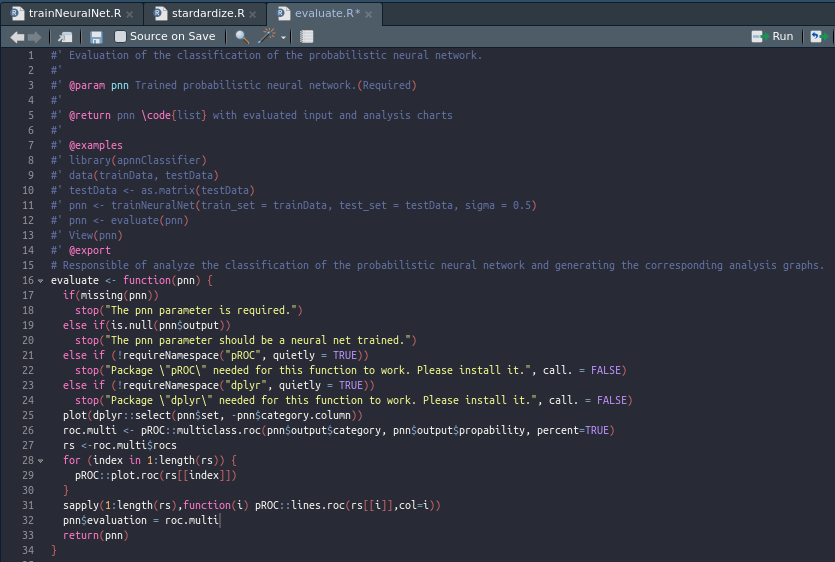
\includegraphics[scale=0.5]{codeEvaluate.png}
	\label{fig:codeEvaluate}
\end{figure}

\item \textbf{Función de estandarización de datos \textit{(standardize)}}, se encarga de estandarizar los datos basado en dos tipos de estandarización para datos discretos o continuos, la codificación de dicha función se muestra en la figura \ref{fig:codeStandardize}. Pag \pageref{fig:codeStandardize}.

\begin{figure}[h]
	\caption{Codificación de la función de estandarización de datos.}
	\centering
	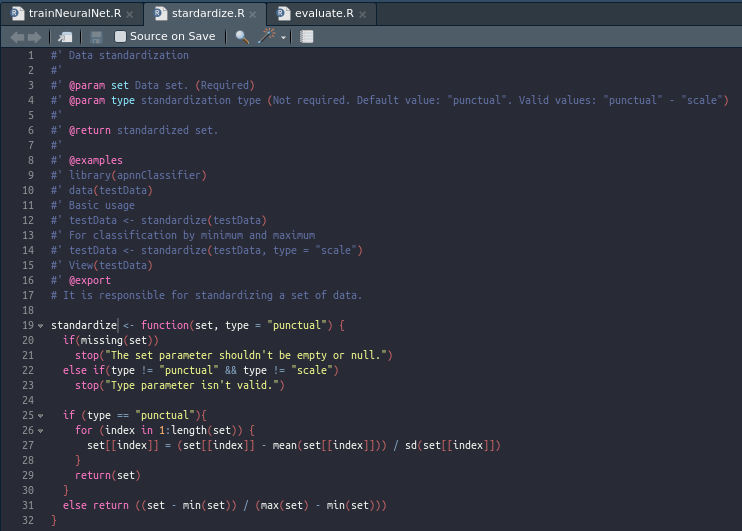
\includegraphics[scale=0.5]{codeStandardize.png}
	\label{fig:codeStandardize}
\end{figure}

\end{itemize}

\section{Chequeo del paquete, método de distribución y registro del método de envío.}

	Para realizar el chequeo del paquete se utilizaron las pruebas unitarias proporcionadas por los paque-
tes R \textit{RUnit} (Zenka, 2015) y \textit{testthat} (Wickham, 2017). Ver figura \ref{fig:check}. Pag \pageref{fig:check}.\\

\begin{figure}[h]
	\caption{Opción check para realizar el chequeo del paquete.}
	\centering
	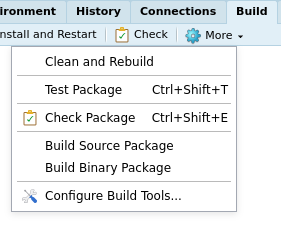
\includegraphics[scale=0.5]{check.png}
	\label{fig:check}
\end{figure}

	Para el metodo de distribución se utilizara \textit{tar.gz}, que es utilizado por defecto por RStudio. Ver figura \ref{fig:build}. Pag \pageref{fig:build}.\\
	

\begin{figure}[h]
	\caption{Opción Build Source Package.}
	\centering
	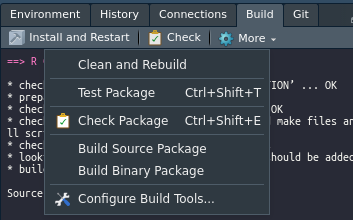
\includegraphics[scale=0.5]{build.png}
	\label{fig:build}
\end{figure}
	
	Como método de envío local se utilizará la plataforma de \textit{GitHub}.\\
	
\section{Pruebas funcionales del paquete}

	El objetivo de este trabajo investigativo consiste en realizar un clasificador de tubérculos de papa criolla para diferentes densidades de siembra y la solución se planteó desarrollando un paquete en R que empleando redes neuronales probabilísticas permitiera dicha clasificación. Para las pruebas funcionales del paquete se realizó la corrida de un algoritmo que permitiera a través del paquete clasificar tubérculos de papa con los datos recogidos en la investigación de Bernal, 2017. \\

	Las características que se tomaron para dicha prueba fueron el diámetro medio ponderado, el peso fresco y la cantidad de papas, encontrándose un total de 2840 datos. Divididos en un 75\% para el set de entrenamiento y un 25\% para el set de pruebas.\\

La codificación del algoritmo se puede observar en la figura \ref{fig:packageuse}. Pag \pageref{fig:packageuse}. \\

\begin{figure}[h]
	\caption{Codificación del algoritmo de clasificación usando \textit{apnnClassifier}.}
	\centering
	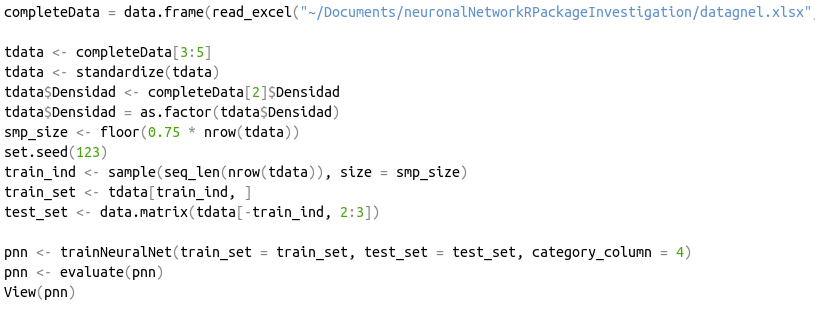
\includegraphics[scale=0.5]{packageuse.png}
	\label{fig:packageuse}
\end{figure}

Los resultados obtenidos por el algoritmo se observan en las figuras \ref{fig:cloudpoints}, Pag \pageref{fig:cloudpoints} - \ref{fig:roc}, Pag \pageref{fig:roc}. \\

\begin{figure}[h]
	\caption{Gráfico de nubes de puntos.}
	\centering
	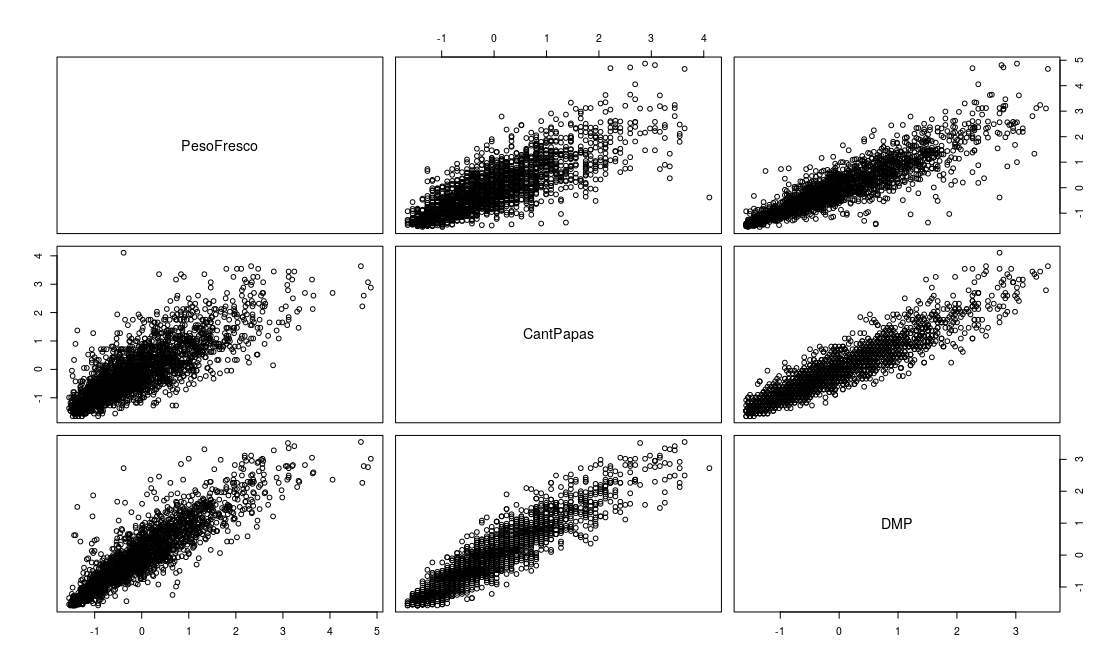
\includegraphics[scale=0.5]{cloudpoints.png}
	\label{fig:cloudpoints}
\end{figure}

\begin{figure}[h]
	\caption{Gráfico de curva característica operativa de receptor.}
	\centering
	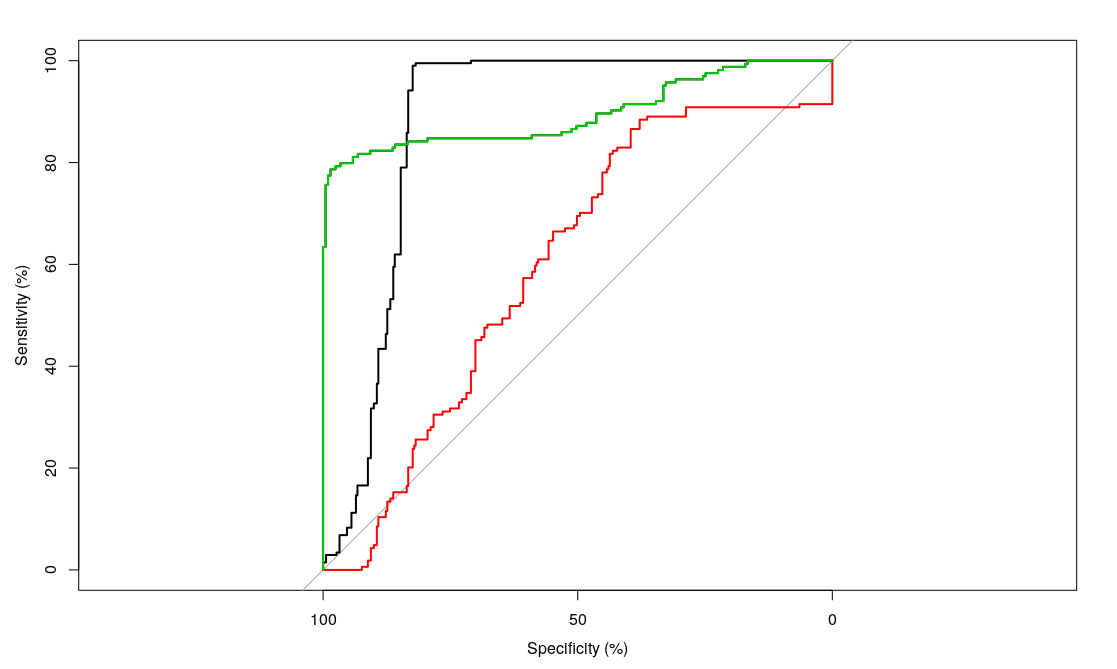
\includegraphics[scale=0.5]{roc.png}
	\label{fig:roc}
\end{figure}